\documentclass[conference]{IEEEtran}
\usepackage{filecontents}
\usepackage[noadjust]{cite}
\usepackage[portuguese]{babel}
\usepackage[utf8]{inputenc}
\usepackage{url}
\usepackage{hyperref}
\usepackage{graphicx}
\usepackage{mathtools}
\usepackage{amsmath}
\usepackage{tikz}
\usepackage{booktabs}
\usepackage{float}
\usepackage{array}
\usetikzlibrary{arrows}
\usepackage[nolist,footnote]{acronym}

\hyphenation{op-tical net-works semi-conduc-tor}    

\title{Redes RBF em problemas de regressão}

\author{\IEEEauthorblockN{Vítor de Albuquerque Torreão}
	\IEEEauthorblockA{Departamento de Estatística e Informática\\
		Universidade Federal Rural de Pernambuco\\
		Recife, Pernambuco\\
		Email: vdat@mail.com}}


\markboth{Disciplina de Redes Neurais, Dezembro~2015}%
{Shell \MakeLowercase{\textit{et al.}}: Bare Demo of IEEEtran.cls for Journals}

\setlength{\heavyrulewidth}{1.5pt}
\setlength{\abovetopsep}{4pt}

\begin{document}
\maketitle

\begin{acronym}
\acro{mlp}[MLP]{Multilayered Perceptron}
\acro{rbf}[RBF]{Radial Basis Function}
\end{acronym}

\begin{abstract}
Dentro da área de modelagem matemática, uma rede de função de base radial (RBF) 
tem como base a teoria convencional de aproximação. Uma rede RBF é uma rede 
neural artificial (RNA) que utiliza funções de base radial como 
funções de ativação dos neurônios. Essas redes constituem uma alternativa 
bastante popular às redes de Perceptron Multicamadas (MLP), por conta de sua 
estrutura mais simples e seu treinamento mais rápido. Essas redes podem ser 
utilizadas em diversos problemas de aprendizado de máquina, tanto de regressão 
como de classificação. Neste artigo, porém, será feito um estudo do potencial 
das redes RBF para resolver exclusivamente problemas de regressão. Serão 
apresentados uma implementação e um estudo de caso para validar o estudo.
\end{abstract}

\begin{IEEEkeywords}
Aprendizado de máquina, redes neurais, regressão
\end{IEEEkeywords}

\section{Introdução}
\label{introducao}

O Perceptron de Múltiplas Camadas, ou \ac{mlp} treinado com o algoritmo \textit{
Backpropagation} \cite{Rumelhart:1988:LIR:65669.104449} é um dos mais 
importantes modelos de Redes Neurais até hoje, devido a sua universal capacidade 
de aproximar funções. Ele é amplamente utilizado em diversos tipos de problemas, 
como regressão, classificação, extração de atributos e memória associativa 
\cite{wu2012using}.

Em 1988, Broomhead e Lowe propuseram o modelo de rede função de base radial, 
também conhecidas como \ac{rbf} \cite{2144306}. Essas redes, da mesma forma que 
as \acp*{mlp} são universais, como mostrado em 
\cite{Park:1991:UAU:110084.110093}, porém exigem um tempo mais curto para o 
treinamento, o que as torna excelentes alternativas.

\subsection{Regressão e Classificação}
\label{regressaoxclassificacao}

Enquanto que problemas de classificação envolvem identificar categorias para 
uma determinada instância no conjunto de dados, regressão está ligada a estimar 
ou prever uma resposta dada como entrada uma instância do conjunto de dados. 
Os dois podem ser diferenciados também pelo fato de que qualquer resposta 
para um problema de classificação é igualmente errada, ao passo que, na 
regressão, existe uma ideia de distância entre as respostas: uma delas pode 
estar mais próxima da resposta correta do que outra. De forma mais simples, 
pode-se dizer que, nos problemas de classificação, as) variáveis de saída 
assumem valores discretos, normalmente, rótulos de classes distintas. Por outro 
lado, nos problemas de regressão, as variáveis de saída assumem valores 
discretos.

Se as variáveis a serem estimadas forem valores futuros, então o procedimento 
sendo construído é um preditor. Caso as variáveis a serem estimadas relacionem 
entradas com saídas, então o procedimento sendo construído é chamado de 
\textit{modelo} \cite{specht1991general}.

Embora tenha sido largamente utilizada na literatura para problemas de 
classificação (\cite{heartrbf}, \cite{wu2012using}, 
\cite{DBLP:conf/isnn/ZhaoYWWL06}), há poucos trabalhos que mostram o potencial 
das redes \ac*{rbf} para problemas de regressão \cite{rojas2002time}. Este 
último será o problema tratado no presente artigo.

\subsection{Estrutura do Texto}
\label{estrutura}

Este trabalho está estruturado da seguinte forma: na seção \ref{relacionados}, 
serão descritos alguns dos trabalhos relacionados ao tema da presente pesquisa; 
na seção \ref{problema} serão apresentados o problema sendo tratado e suas 
principais características; na seção \ref{rbf} serão apresentadas as redes 
\ac*{rbf}; na seção \ref{resultados} serão mostrados alguns dos resultados 
obtidos para problemas de regressão utilizando \acp*{rbf} na seção 
\ref{trabalhos_futuros} serão apresentados alguns dos possíveis trabalhos a 
serem derivados a partir desta pesquisa; por fim, a seção \ref{conclusao} 
conclui este trabalho com algumas considerações finais.

\section{Trabalhos Relacionados}
\label{relacionados}
Nesta seção serão apresentados alguns trabalhos encontrados na literatura que 
apresentam relação com a presente pesquisa e podem ser relevantes para entender 
o contexto e motivações para sua realização.

Em ambos \cite{orr1996introduction} e \cite{borsintroduction} fazem uma 
introdução para as redes neurais \ac*{rbf}. Os autores descrevem as principais 
propriedades focando na topologia e arquitetura, além de apresentar algumas das 
motivações para seu uso e aplicações.

\cite{wu2012using} discute algumas aplicações para as redes \ac*{rbf}, variando 
de aplicações em visão computacional e modelagem de sistemas dinâmicos até 
redes neurais \ac*{rbf} para sistemas com valores complexos. O objetivo do 
trabalho é apresentar as \acp*{rbf} como alternativas para as \acp*{mlp} 
principalmente para problemas de aproximação de função e classificação.

Em \cite{heartrbf}, redes neurais \ac*{rbf} e de Regressão Generalizada são 
utilizadas na tarefa de diagnosticar doenças do cardíacas e prescrever os 
remédios necessários. O trabalho conclui que os resultados encontrados pela 
aplicação das redes \ac*{rbf} são satisfatórios, tendo, inclusive, validado 
com médicos.

Em \cite{rojas2002time}, é proposto um \textit{framework} para construir e 
treinar redes neurais \ac*{rbf}. Um algoritmo de aprendizado sequencial é 
apresentado para adaptar a estrutura da rede, sendo possível criar novas 
unidades na camada escondida, além de detectar e remover neurônios inativos.
Mesmo tendo como foco a apresentação do inovador \textit{framework}, o trabalho 
demonstra as vantagens do seu novo algoritmo de treinamento sequencial, através 
dos resultados das redes treinadas para o problema de predizer séries temporais.

Pode-se observar dos trabalhos relacionados que o uso extensivo das redes 
\ac*{rbf} para problemas de classificação deixa uma lacuna a ser investigada: 
se redes \ac*{rbf} são boas alternativas para problemas de regressão.

\section{O Problema}
\label{problema}

O problema de regressão \cite{specht1991general} pode ser definido da seguinte 
forma: para uma determinada variável, $Y$, dependente em uma variável, $X$, 
independente, é a computação do valor mais provável de $Y$ para cada valor de 
$X$, tendo como base apenas um número finito de medições de $X$ (possivelmente 
com ruídos) e seus respectivos valores de $Y$. Essas variáveis $X$ e $Y$ são, 
normalmente, vetores. No sistema, a variável dependente, $Y$, é a saída, 
enquanto que a variável independente, $X$ é a entrada.

Observe, por exemplo, a figura \ref{fig:regressao}. Ela representa um 
exemplo de tais dados, com os valores de $X$ e $Y$ nos eixos.

\begin{figure}[t]
	\caption{Exemplo de dados disponíveis para regressão.}
	\label{fig:regressao}
	\centering
	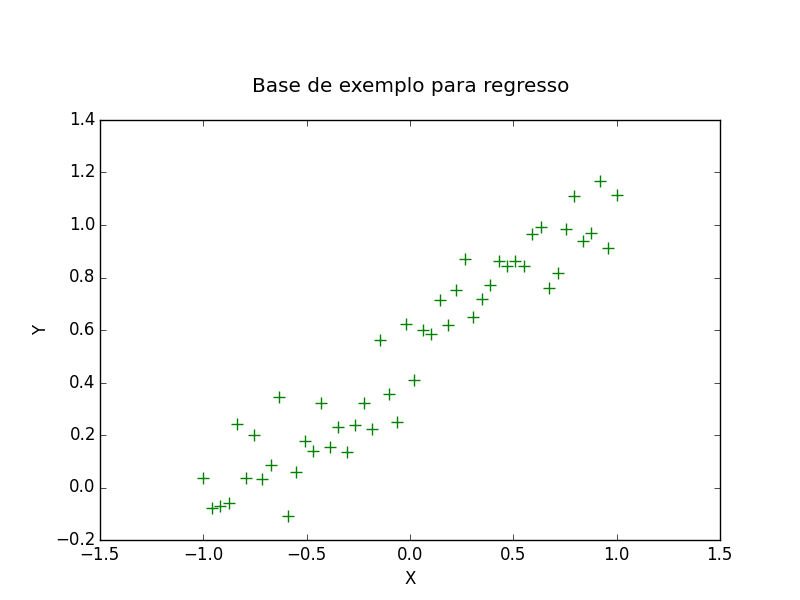
\includegraphics[width=0.40\textwidth]{regression_data_example}
\end{figure}

Para implementar uma solução é, normalmente, necessário assumir alguma função 
com parâmetros desconhecidos $a_{i}$. Os valores desses parâmetros são então 
calibrados para melhor ajuste da função aos dados observados. No caso da 
regressão linear, por exemplo, a saída é assumida como uma função linear da 
entrada, e assim, os parâmetros desconhecidos, $a_{i}$ seriam os coeficientes 
lineares da função.

Ou seja, o problema de regressão pode ser resumido em encontrar um modelo capaz 
de prever corretamente (ou com menor erro possível) o valor da saída do sistema
através do ajuste de parâmetros internos do modelo. A entrada para esse ajuste é 
um conjunto $\{x_{i}, \hat{y}_{i}\}_{i=1}^{p}$. Onde $x_{i}$ é o valor da 
$i$-ésima observação da variável independente $X$ e $\hat{y}_{i}$ é o valor da 
variável dependente $Y$, dado o valor de $X$.

No decorrer deste trabalho, esse problema será tratado utilizando redes neurais 
\acp*{rbf} para relacionar a entrada, $X$ e a saída, $Y$.

\section{Redes RBF}
\label{rbf}

As Redes \ac*{rbf} são redes neurais artificiais \textit{feed-foward} de 
múltiplas camadas. Elas possuem, em geral, uma camada de entrada, uma camada 
neural escondida e uma camada neural de saída \cite{wu2012using}. A figura 
\ref{fig:rbf} detalha melhor a arquitetura dessas redes.

\begin{figure}[t]
	\caption{Configuração típica da rede \ac*{rbf}}
	\centering
	\vspace*{19pt}
	\begin{tikzpicture}[every node/.style={circle, draw=black, minimum size=17pt,inner sep=0pt}]
	
	\tikzset{edge/.style = {->,> = latex'}}
	
	\node (1)  at (0,4)   {$x_{1}$};
	\node (2)  at (0,2)   {$x_{2}$};
	\node[draw=white] (3)  at (0,1)   {...};
	\node (4)  at (0,0)   {$x_{n}$};
	
	\node (5)  at (2,4)   {$u_{1}$};
	\node (6)  at (2,2)   {$u_{2}$};
	\node[draw=white] (7)  at (2,1)   {...};
	\node (8)  at (2,0)   {$u_{n_{1}}$};
	
	\node (9)  at (4,3)   {$u_{1}$};
	\node[draw=white] (10)  at (4,2)   {...};
	\node (11)  at (4,1)   {$u_{n_{2}}$};
	
	\node[draw=white] (12)  at (5,3.5) {$-\theta_{1}$};
	\node[draw=white] (13)  at (5,1.5) {$-\theta_{n_{2}}$};
	
	\foreach \source/\dest in {1/5,1/6,1/8,2/5,2/6,2/8,4/5,4/6,4/8,5/9,5/11,6/9,6/11,8/9,8/11,12/9,13/11}
	\draw[edge] (\source) to (\dest);
	
	\end{tikzpicture}
	\label{fig:rbf}
\end{figure}

As grandes diferenças entre as \acp*{rbf} as redes \ac*{mlp} estão na função de 
ativação e no treinamento da camada neural escondida \cite{daredes}.

As funções de ativação utilizadas nos neurônios da camada escondida são 
justamente aquelas que dão nome ao algoritmo: as funções de base radial. Dentre 
elas, a mais utilizada é a função gaussiana \cite{gaussian}, dada pela expressão 
abaixo e ilustrada na figura \ref{fig:gaussian}.

$$g(u) = e^{-\frac{(u-c)^{2}}{2\sigma^{2}}}$$

Onde $c$ define o centro da função gaussiana e $\sigma^{2}$ denota a variância.

Já o treinamento das redes \ac*{rbf} é dividido em duas fases: uma fase não 
supervisionada e uma supervisionada \cite{daredes}. Na primeira fase do 
treinamento, são ajustados os pesos dos neurônios da camada escondida, que 
efetivamente correspondem ao parâmetro $c$ da função gaussiana. Isso significa 
que quanto mais próxima do centro de um determinado neurônio uma instância 
estiver, maior será a saída daquele neurônio para aquela entrada.

Um dos métodos mais utilizados para calcular os centros das gaussianas é o 
algoritmo $k$-\textit{means} \cite{daredes}. O parâmetro $k$ desse algoritmo 
será precisamente o número de neurônios na camada escondida. Nesta pesquisa 
foi utilizado este algoritmo para o treinamento não supervisionado.

Só depois que a etapa não supervisionada estiver completa, é iniciada a última 
fase. Nesta etapa é feito um treinamento supervisionado utilizando a regra delta 
generalizada para ajustar os pesos dos neurônios da camada de saída de forma 
similar ao treinamento da rede \ac*{mlp} \cite{daredes}.

Para problemas de classificação, a saída da rede é, normalmente, uma das 
possíveis classes presentes no problema na qual a instância de entrada deve 
pertencer segundo o modelo, ou seja, a saída é um valor discreto. Mas para 
problemas de regressão, a saída é o valor da variável dependente ($Y$) 
encontrada pelo modelo, ou seja, um valor contínuo. Neste trabalho foi 
utilizada a função linear como função de ativação dos neurônios na camada de 
saída.

\begin{figure}[t]
	\caption{Função gaussiana com $\sigma^{2} = 0.05$ e $c = 0$}
	\label{fig:gaussian}
	\centering
	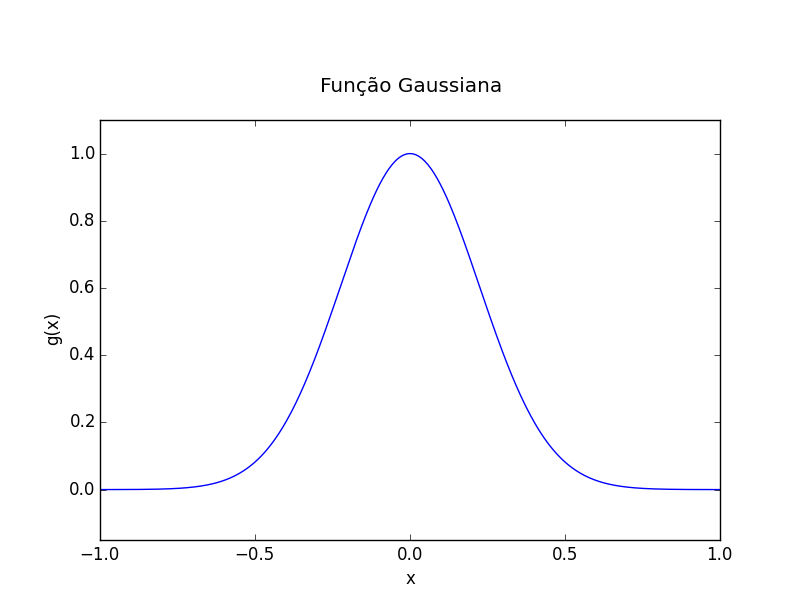
\includegraphics[width=0.40\textwidth]{gaussian}
\end{figure}

\section{Regressão com redes RBF}
\label{resultados}

\begin{table*}[t]
	\centering
	\caption{Resultados obtidos}
	\label{corrmatrix}
	\begin{tabular}{l c c l c c l c c}
		\toprule
		Logística & & & Seno & & & Cosseno & & \\
		\midrule
		{} & 3 & 0.001500 & {} & 3 & 0.095880 & {} & 3 & 0.011652 \\
		{} & 4 & 0.000588 & {} & 4 & 0.006498 & {} & 4 & 0.000908 \\
		{} & 5 & 0.000443 & {} & 5 & 0.002339 & {} & 5 & 0.001868 \\
		{} & 6 & 0.000265 & {} & 6 & 0.001677 & {} & 6 & 0.000469 \\
		{} & 7 & 0.000483 & {} & 7 & 0.000614 & {} & 7 & 0.000722 \\
		{} & 8 & 0.000370 & {} & 8 & 0.000548 & {} & 8 & 0.000572 \\
		{} & 9 & 0.001110 & {} & 9 & 0.000392 & {} & 9 & 0.000386 \\
		{} & 10 & 0.000721 & {} & 10 & 0.000901 & {} & 10 & 0.000218 \\
		\bottomrule
	\end{tabular}
\end{table*}


\begin{figure}[b]
	\caption{Dados para base de treinamento obtidos através da aplicação de 
		ruído na função seno}
	\label{fig:seno_dados}
	\centering
	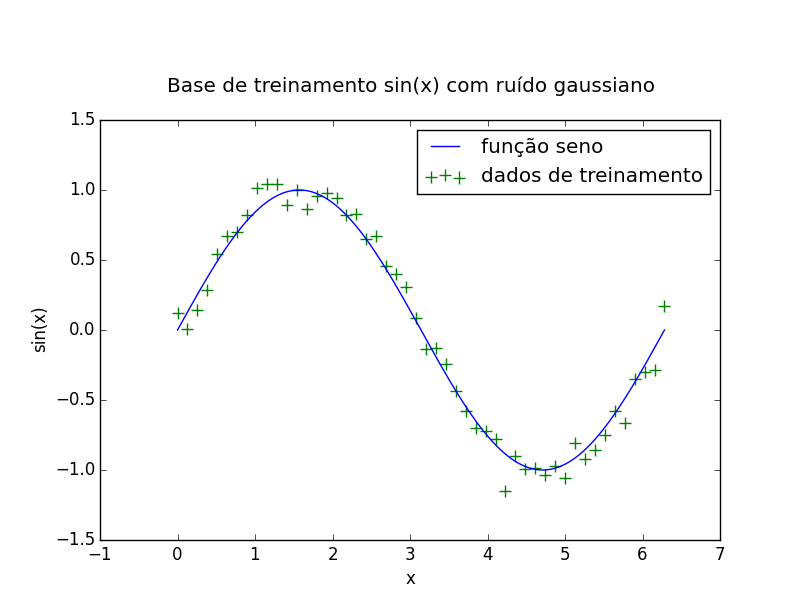
\includegraphics[width=0.40\textwidth]{sin_5v1_train_data_paper}
\end{figure}

Dadas as configurações explanadas na seção \ref{fig:rbf}, esta seção visa 
ilustrar os resultados obtidos para problemas de regressão utilizando redes 
\ac*{rbf}.

Para isso, foram construídas três bases de dados. Na primeira, foram 
calculados cinquenta pontos entre $0$ e $2\pi$. Para cada ponto, $x$, assim 
definido, foi aplicada a função seno e a esse valor foi adicionado um pequeno 
ruído gaussiano. De forma que, para cada $x$, temos um $y = sen(x) + 
\epsilon$, onde $\epsilon$ é um valor aleatório provido de uma distribuição 
normal. Como resultado, foi obtida a base ilustrada na figura 
\ref{fig:seno_dados}. Na segunda base, o mesmo processo foi feito para a função 
cosseno, ou seja, para cada $x$ temos que $y = cos(x) + \epsilon$ e o 
resultado está na figura \ref{fig:cosseno_dados}.

Por fim, para a última base de dados, foram calculados cinquenta pontos entre 
$-1$ e $1$. Para cada ponto, $x$, foi aplicada a função logística \cite{logist} 
definida abaixo:

$$f(x) = \frac{L}{1 + e^{-k(x-x_{0})}}$$

Onde $L$ é o maior valor da curva, $x_{0}$ é o valor, no eixo $X$, do ponto 
médio da sigmoide e $k$ representa a declividade da curva. Foram utilizados os 
valores $L = 1$, $k = 4$ e $x_{0} = 0$.

Além de aplicada a função logística para cada $x$ também foi adicionado um 
pequeno ruído gaussiano. Assim, para um dado valor de $x$, $y = f(x) + 
\epsilon$, onde $\epsilon$ é um valor aleatório provido por uma distribuição 
normal. Os pontos dessa base podem ser visualizados na figura 
\ref{fig:logistica}.

\begin{figure}[t]
	\caption{Dados para base de treinamento obtidos através da aplicação de 
		ruído na função cosseno}
	\label{fig:cosseno_dados}
	\centering
	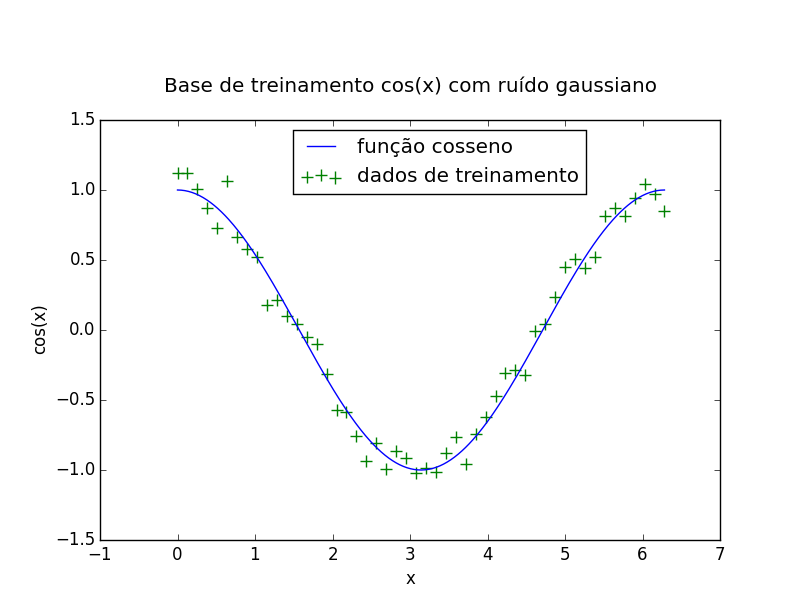
\includegraphics[width=0.40\textwidth]{cos_5v1_train_data_paper}
\end{figure}

\begin{figure}[b]
	\caption{Dados para base de treinamento obtidos através da aplicação de 
		ruído na função cosseno}
	\label{fig:logistica}
	\centering
	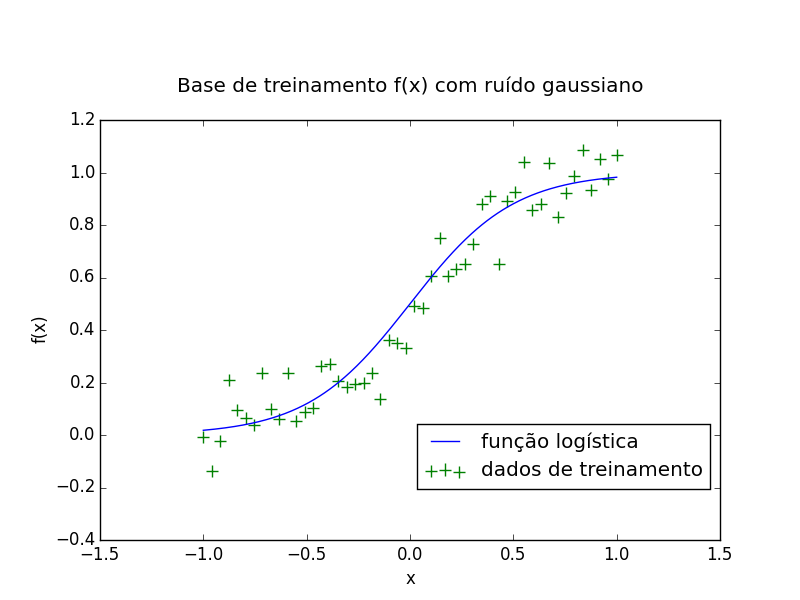
\includegraphics[width=0.40\textwidth]{f_5v1_train_data_paper}
\end{figure}


Uma vez que as bases estavam montadas, elas foram utilizadas para treinar uma 
rede neural \ac*{rbf}. Uma vez que o treinamento foi finalizado, esse modelos 
foram utilizados para calcular o valor esperado de $y$, para cada uma das três 
funções. Porém, para estas avaliações, foram utilizados quatrocentos valores ao 
invés de apenas cinquenta. Além disso, o número de neurônios na camada escondida 
foi variado entre 3 e 5. A métrica utilizada para avaliação foi o erro 
quadrático médio definido por \cite{daredes} da seguinte forma: 

$$E_{M} = \frac{1}{p}\sum_{k=1}^{p}\frac{1}{2}\sum_{i=1}^{n_{2}}
(d_{j}(k)-y_{j}^{2}(k))^{2}$$

Onde $p$ é o número de amostras, $n_{2}$ é o número de neurônios na camada de 
saída, $d_{j}(k)$ é a saída correta do $j$-ésimo neurônio da camada de saída 
para a $k$-ésima amostra  e $y_{j}^{2}(k)$ é a saída obtida pelo $j$-ésimo 
neurônio da camada de saída para a amostra $k$.

Os resultados obtidos estão sumarizados na tabela \ref{tbl:resultados}. 
Ilustrações dos modelos encontrados estão disponíveis nas figuras 
\ref{fig:rsl_seno}, \ref{fig:rsl_cos} e \ref{fig:rsl_logistic}.

Olhando estes resultados, pode-se concluir primeiramente que as redes \ac*{rbf} 
foram muito bem em capturar a relação entre a variável independente $X$ e a 
variável dependente $Y$.

Além disso, é possível perceber que para a base feita com a função logística, 
aumentar o número de neurônios na camada escondida para além de seis, não trouxe 
melhores resultados. Para a base feita a partir da função seno observa-se uma 
considerável acentuação do erro quadrático médio na mudança de nove para dez 
neurônios, porém, seriam necessários mais experimentos para ter certeza que 
essa tendência se mantém a medida que o número de neurônios sobem. Já para a 
base feita com a função cosseno, valeu a regra de quanto mais neurônios, 
melhor o resultado, pelo menos até dez neurônios.

Por fim, é importante notar que a base que apresentou a maior dificuldade para 
as redes \ac*{rbf} foi a base montada a partir da função seno.

\section{Trabalhos Futuros}
\label{trabalhos_futuros}

Ficam como trabalhos futuros desta pesquisa realizar mais experimentos para 
entender melhor a relação entre a quantidade de neurônios e a variação no erro 
quadrático médio encontrado.

Também seria interessante, utilizar outras bases de dados de problemas de 
regressão para verificar a performance das redes \ac*{rbf}. Por exemplo, 
poderiam ser utilizadas bases de problemas do mundo real, como a de previsão 
de subida/descida da bolsa de valores ou de preços de imóveis.

\section{Conclusão}
\label{conclusao}

Os problemas de regressão se mostram bastante desa

\section*{Agradecimentos}
We acknowledge the acknowledged acknowledgees.


\bibliography{artigo}
\bibliographystyle{IEEEtran}

\end{document}